% =========================================================================== %
% Introduction
% =========================================================================== %

\ifx\wholebook\relax\else
  \documentclass[a4paper,10pt,twoside]{book}
  %=============================================================================%
% Common things, settings, packages to include
%=============================================================================%

\usepackage{graphicx}
\usepackage{color}
\usepackage{makeidx}
\usepackage{ifpdf}
\usepackage{verbatim}

% --------------------------------------------------------------------------- %
% Setting up stuff depeding on output format
% --------------------------------------------------------------------------- %

\ifpdf
  % special settings for pdf mode
  \usepackage[colorlinks]{hyperref}
  \usepackage{courier}
  
  \hypersetup{
    colorlinks,
    linkcolor=darkblue,
    citecolor=darkblue,
    pdftitle={The Eclipse Scout Book},
    pdfauthor={The Scout Community},
    pdfkeywords={Enterprise Framework, Eclipse, Java, Client-Side, Rich Client, Web Client, Mobile},
    pdfsubject={Computer Science}
  }
  
  \usepackage{caption}
  \captionsetup{margin=10pt,font=small,labelfont=bf}
\else
  % special stuff for html mode
  \usepackage[tex4ht]{hyperref}
\fi

% --------------------------------------------------------------------------- %
% Setting up printing range
% --------------------------------------------------------------------------- %

\parindent 1cm
\parskip 0.2cm
\topmargin 0.2cm
\oddsidemargin 1cm
\evensidemargin 0.5cm
\textwidth 15cm
\textheight 21cm

% --------------------------------------------------------------------------- %
% Setting up listings
% --------------------------------------------------------------------------- %

\usepackage{listings}
 
\definecolor{darkviolet}{rgb}{0.5,0,0.4}
\definecolor{darkgreen}{rgb}{0,0.4,0.2} 
\definecolor{darkblue}{rgb}{0.1,0.1,0.9}
\definecolor{darkgrey}{rgb}{0.5,0.5,0.5}
\definecolor{lightblue}{rgb}{0.4,0.4,1}
\definecolor{lightgray}{rgb}{0.97,0.97,0.97}

\renewcommand{\lstlistlistingname}{List of Listings}

% general settings
\lstset{
  basicstyle=\small\ttfamily,
  columns=fullflexible,
  breaklines=true,
  breakindent=10pt,
  prebreak=\mbox{{\color{blue}\tiny$\searrow$}},
  postbreak=\mbox{{\color{blue}\tiny$\rightarrow$}},
  showstringspaces=false,
  backgroundcolor=\color{lightgray}
}

% settings for xml files
\lstdefinelanguage{xml}
{
  commentstyle=\color{darkgrey}\upshape,
  morestring=[b]",
  morestring=[s]{>}{<},
  morecomment=[s]{<?}{?>},
  stringstyle=\color{black},
  identifierstyle=\color{darkblue},
  keywordstyle=\color{cyan},
  morekeywords={xmlns,name,point,factory,class}% list your attributes here
}

% settings for ini files
\lstdefinelanguage{ini}
{
  morecomment=[f][\color{darkgrey}\upshape][0]\#, % # is comment iff it's the first char on the line
  stringstyle=\color{black}
}

% default settings (for java files)
\lstset{
  language=Java,
  emphstyle=\color{red}\bfseries,
  keywordstyle=\color{darkviolet}\bfseries,
  commentstyle=\color{darkgreen},
  morecomment=[s][\color{lightblue}]{/**}{*/},
  stringstyle=\color{darkblue},
}

% --------------------------------------------------------------------------- %
% cross reference macros
% --------------------------------------------------------------------------- %
\newcommand{\applabel}[1]{\label{apx:#1}}
\newcommand{\chalabel}[1]{\label{cha:#1}}
\newcommand{\seclabel}[1]{\label{sec:#1}}
\newcommand{\lstlabel}[1]{\label{lst:#1}}
\newcommand{\figlabel}[1]{\label{fig:#1}}
\newcommand{\tablabel}[1]{\label{tab:#1}}

\newcommand{\appref}[1]{Appendix~\ref{apx:#1}}
\newcommand{\charef}[1]{Chapter~\ref{cha:#1}\xspace}
\newcommand{\secref}[1]{Section~\ref{sec:#1}}
\newcommand{\lstref}[1]{Listing~\ref{lst:#1}\xspace}
\newcommand{\figref}[1]{Figure~\ref{fig:#1}\xspace}
\newcommand{\tabref}[1]{Table~\ref{tab:#1}\xspace}

% --------------------------------------------------------------------------- %
% graphics paths
% --------------------------------------------------------------------------- %
\graphicspath{
  {figures/}
  {Introduction/figures/}
}

%=============================================================================%

  \pagestyle{headings}
  \graphicspath{{figures/} {../figures/}}
  \begin{document}
  \sloppy
\fi


% =========================================================================== %
\chapter{Introduction}

% --------------------------------------------------------------------------- %
\section{What is Eclipse Scout?}

\fbox{
  \parbox{12cm}{
    Section waiting for contribution (max 2'000 words)
	
    The focus of the first section should be on benefits of Scout.
	History should point to the 10 years of existence of Scout and previous technology transitions.
	Outlook should focus on values such as stability, dedication to grow the community and moving with best available technolgies.
  }
}

\noindent Existing Documentation
\begin{itemize}
  \item concept wiki \url{http://wiki.eclipse.org/Scout/Overview}
\end{itemize}

\subsection{Benefits of Scout}

\noindent Existing Documentation
\begin{itemize}
  \item concept wiki \url{http://wiki.eclipse.org/Scout/Overview/Why_You_Should_Use_Scout}
\end{itemize}

Eclipse Scout is a mature and open framework for modern, 
service oriented business applications.

With its multi-frontend support, Scout applications may run as desktop 
applications, in the web or on a mobile using a single codebase.

Scout substantially boosts developer productivity and is simple to learn.

User friendly applications are straight forward to implement with Scout�s 
comprehensive set of user interface components.

Completely based on Java/Eclipse, Scout Applications are easy to integrate 
in most IT environments.

\subsection{A short History}
needs text

\subsection{Outlook}
needs text

\newpage

% --------------------------------------------------------------------------- %
\section{What should I read?} 
\seclabel{whatshouldiread}

The text below provides guidelines on what to read (or what to skip) depending on your existing background.

We first address the needs of junior Java developers that like to learn more about developing enterprise applications.
Then, we suggest a list of sections relevant for software wizards that already have a solid understanding of the Eclipse platform, Java enterprise technolgies, and real world applications.
Finally, the information needs of IT managers are considered.

% ........................................................................... %
\subsection{I know some Java}

The good news first.
This book is written for you! 
No prior knowledge of the Eclipse Platform\footnote{Eclipse Platform: \url{http://wiki.eclipse.org/Platform}} is needed. 
We do not even assume that you have a meaningful understanding of the Java Enterprise Edition 
(Java EE)\footnote{Java Enterprise Edition: \url{http://en.wikipedia.org/wiki/Java_Platform,_Enterprise_Edition}}.
Of course, having prior experience in client server programming with Java is helpful.
It also helps having used the Eclipse IDE for Java development before --- please do not mistake the IDE with the Eclipse 
platform\footnote{By reading through the book you will learn that there is much more to the Eclipse platform than just the IDE}.
However, prior knowledge of Java EE and the Eclipse platform is not required for this book.

The ``bad'' news is, that writing Scout applications requires a solid understanding of Java.
To properly benefit from this book, we assume that you have been developing software for a year or more.
And you should have masterd the Java Standard Edition 
(Java SE)\footnote{Java Standard Edition: \url{http://en.wikipedia.org/wiki/Java_SE}} to a significant extent. 
To be more explicit, you are expected to be comfortable with all material required for the Java Programmer Level I 
Exam\footnote{Level I Exam: \url{docs.oracle.com/javase/tutorial/extra/certification/javase-7-programmer1.html}}
and most of the material required for 
Level II\footnote{Level II Exam: \url{docs.oracle.com/javase/tutorial/extra/certification/javase-7-programmer2.html}}.

As the focus of this book is on writing Scout applications and not on learning Java, Java EE, or the Eclipse platform, the necessary background material has been moved into corresponding appendices.
To get a more precise picture which parts of Java and Eclipse are important to Scout applications, consult the appendices listed below.

\begin{itemize}
  \item \appref{java_basics} highlighs relevant advanced Java SE concepts and necessary Java EE topics. 
        In addition, the appendix contains recommendations for introductory material as well as pointers to further reading regarding Java EE technology.
  \item \appref{eclipse_basics} provides a brief introduction for Eclipse concepts used in Scout. 
        This includes the OSGi/Equinox foundation as well as additional elements such as Eclipse plugins, feature and product files.
\end{itemize}

We now propose to start downloading and installing Scout as described in \appref{install_scout} and do some actual coding.
To do so, please continue with the ``Hello World'' example provided in \charef{helloworld}.
You can expect to complete this example in less than two hours including the necessary download and installation steps.
Afterwards, you might want to continue with the remaining material in ``Getting Started''. 
Working through the complete ``Getting Started'' should take no more than two days. 
This exercise will provide you with a broad overview of Eclipse Scout and enough hands-on material to decide how much Scout will help you with your current and future projects.

How you continue after ``Getting Started'' will depend on your current interests or your specific project. 
``The Frontend'' and ``The Backend'' walk you through the Scout application model covering the client, the server, and the necessary communication in the context of a typical business application.
``Developing Applications'' contains additional Scout features, relevant aspects for integrating Scout applications in an enterprise envrionment, and typical topics important to professional software development.

Once you work with the Scout framework on a regular basis, you might want to ask questions in the Scout 
forum\footnote{Eclipse Scout forum: \url{http://www.eclipse.org/forums/eclipse.scout}}.
When your question gets answered, please ask yourself if your initial problem could have been solved by better documentation.
In that case, you might want to help the Scout community by fixing or amending the Scout wiki pages\footnote{Eclipse Scout wiki: \url{http://wiki.eclipse.org/Scout}}.
Or this book. 
If you find a bug in Eclipse Scout that makes your life miserable you can report it. 
When your bug is fixed, you can test the fix.
To help speed up the bugfixing process you can contribute patches.
All of these actions will add to the healthy grow of the Scout community.
And this is exactly the topic of ``Contributing'', the last part of this book.

% ........................................................................... %
\subsection{I know tons of both Java and Eclipse}

This means that you are one of these software wizards that get easily bored.
You probably hate going through lengthy descriptions of widely known concepts.
In that case let us assume that you are prepared to spend two hours to grasp the scope of Eclipse Scout and get an impression of its strengths and limitations.

In that case you will not need to actually download, install, and code. 
Rather, it will suffice to flip through a couple of diagrams and screenshots, read about some central Scout concepts, and look at some code snippets provided in this book.
The list below suggests a sequence of sections to digest including a brief motivation for each one.

\begin{itemize}
  \item read ''getting started'' but skip the larger example
  \item read overview and client modeling in frontend 
  \item flip though the form fields provided out of the box
  \item maybe check custom fields to see how to add missing form fields
  \item read overview and transaction management in backend
  \item read application extensions to learn how scout applications can be properly modularized 
  \item maybe check how to use your favorite logging framework with scout
  \item glance at web and mobile application to learn how scout can use a single codebase to run an application on the desktop in the web, and on mobile devices
  \item glance over the shocase sections in "integrating 3rd party" to see how scout applications integrate with other frameworks
  \item flip though testing/profiling to convince yourself that developing scout applications is not different from developing other java/eclise applications	
\end{itemize}

% ........................................................................... %
\subsection{I am a manager}

Beeing a manager and actually reading this book may indicate one of the following situations:

\begin{itemize}
  \item Your developer tried to convince you that Eclipse Scout can help you with implementing business applications in a shorter time and for less money.
        And you did not understand why (again) a new technology should work better than the ones you already use. 
	
\end{itemize}

% =========================================================================== %
\chapter{"Hello World"}
\chalabel{helloworld}

needs text

\noindent Existing Documentation
\begin{itemize}
  \item wiki tutorial \url{http://wiki.eclipse.org/Scout/Tutorial/3.8/HelloWorld}
\end{itemize}

% --------------------------------------------------------------------------- %
\section{Installation and Setup}
needs text

% --------------------------------------------------------------------------- %
\section{Creating a new Application}
needs text

\noindent Existing Documentation
\begin{itemize}
  \item how-to wiki \url{http://wiki.eclipse.org/Scout/HowTo/3.8/Create_a_new_project}
\end{itemize}

% --------------------------------------------------------------------------- %
\section{The User Interface Part}
needs text

\begin{figure}
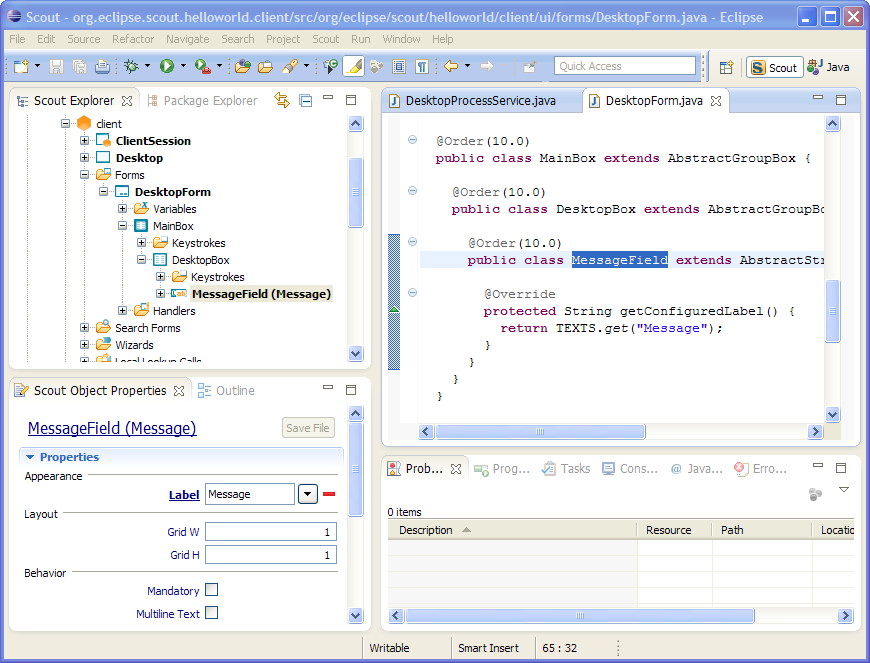
\includegraphics[width=15cm]{sdk_helloworld_messagefield.png}
\caption{Scout SDK showing the \it{MessageField}}
\figlabel{helloworld_messagefield}
\end{figure}


% --------------------------------------------------------------------------- %
\section{The Server Part}
needs text

here comes a listing

\lstinputlisting[
  label=lst:helloworld.load,
  caption=Assigning "hello world" to the form data's message field.,
  index={DesktopFormData,DesktopProcessService},
  emph={getMessage,setValue},
  linerange={10-14},
  float
]
{../code/helloworld/org.eclipse.scout.helloworld.server/src/org/eclipse/scout/helloworld/server/services/process/DesktopProcessService.java}

% --------------------------------------------------------------------------- %
\section{Running the Application}
needs text

\noindent Existing Documentation
\begin{itemize}
  \item wiki tutorial \url{http://wiki.eclipse.org/Scout/Tutorial/3.8/HelloWorld#Run_the_.22hello_world.22_application}
\end{itemize}

% --------------------------------------------------------------------------- %

\ifx\wholebook\relax\else
   \begin{thebibliography}{99}
  \addcontentsline{toc}{chapter}{Bibliography}
  
  % add/insert books in alphabetical order of 1st author
  
  \bibitem{batessierra05}
    \textit{Bert Bates, Kathy Sierra},
	\textbf{Head First Java} 2nd edition, 
	O'Reilly Media, 2005.

  \bibitem{bloch08} 
    \textit{Joshua Bloch},
    \textbf{Effective Java} 2nd edition, 
	Addison-Wesley, 2008.
	
  \bibitem{eckel06}
    \textit{Bruce Eckel},
	\textbf{Thinking in Java} 4th edition, 
	Prentice Hall International, 2006.

\end{thebibliography}

   \end{document}
\fi

% =========================================================================== %
